\documentclass[preprint,12pt]{elsarticle}

\usepackage[T1]{fontenc}
\usepackage{lmodern}
\IfFileExists{glyphtounicode.tex}{\input{glyphtounicode}\pdfgentounicode=1}{}
\usepackage{amsmath}
\usepackage{amsthm}
\usepackage{booktabs}
\usepackage{graphicx}
\usepackage[protrusion=true,expansion=false]{microtype}
\usepackage{xurl}
\usepackage{placeins}
\newtheorem{proposition}{Proposition}
\setlength{\emergencystretch}{2em}

\journal{Applied Soft Computing}

\begin{document}

\begin{frontmatter}

\title{Support-Aware Neuro-Memory Reinforcement Learning under Support Shift:
A Soft-Computing Boundary Analysis}

\author[inst1]{Ercan Erkalkan\corref{cor1}}
\cortext[cor1]{Corresponding author}
\ead{ercan.erkalkan@marmara.edu.tr}
\ead[url]{https://orcid.org/0000-0001-9259-7112}
\address[inst1]{Vocational School of Technical Sciences, Department of
Electronics and Automation, Artificial Intelligence Operator Program,
Marmara University, Mehmet Gen\c{c} Campus, 34865 Kartal, Istanbul, Turkey}

\begin{abstract}
Hybrid neuro-memory reinforcement learning must arbitrate between transparent
exact-state evidence and neural estimates that can extrapolate beyond observed
support. We present a reproducible soft-computing boundary analysis of
tabular--neural Q-learning, including a fuzzy support- and uncertainty-aware
gate and a controlled application-inspired navigation case with deployment
goal shift. Experiments retain seed-level outcomes, exact environment-step
checkpoints, isolated evaluation randomness, and explicit separation of
development, confirmation, diagnosis, and replication. The navigation study
uses 30 matched seeds and reports return area under the learning curve (AUC),
success, collision, unsupported-state ratio, branch use, abstention,
exact-memory size, and decision time. The fuzzy gate improves application AUC
over the validated deep Q-network (DQN) by 0.575 (bootstrap 95\% interval
[0.152, 0.987]) but is worse than tabular Q-learning and safe support
abstention. Across compact validation, it improves over DQN on FrozenLake 4x4
and under Wilcoxon sensitivity on CliffWalking, but it does not significantly
outperform count gating. At complete held-out support, its zero-support neural
fallback reproduces the count gate's failure, whereas abstention avoids
unsupported neural preferences. Fuzzy arbitration also adds measurable
decision-time overhead. The contribution is therefore not a universally
superior algorithm, but an auditable pre-deployment diagnostic: exact memory
helps when states recur, adaptive arbitration helps only when its reliability
signals are informative, and explicit fallback remains necessary at the
support boundary.
\end{abstract}

\begin{keyword}
reinforcement learning \sep neuro-memory \sep fuzzy arbitration \sep
deep Q-network \sep support shift \sep abstention \sep soft computing
\end{keyword}

\end{frontmatter}

\section{Introduction}
\label{sec:introduction}

Tabular Q-learning stores an independently updated action value for each
observed state \cite{watkins1992qlearning}. This representation is transparent
and rapidly correctable when exact states recur, but it has no mechanism for
generalizing to an unseen state. Deep Q-networks (DQN) replace the table with a
function approximator and use replay and target networks to stabilize
learning \cite{mnih2015dqn,vanhasselt2016double}. The substitution enables
generalization while introducing optimization sensitivity, target error, and
seed-dependent evaluation uncertainty
\cite{henderson2018matters,agarwal2021precipice}.

From a soft-computing perspective, this tension is central rather than
incidental. Soft computing emphasizes approximate reasoning and adaptive
computation under imprecision, uncertainty, and partial evidence
\cite{zadeh1994soft}. A reinforcement-learning controller that acts in states
outside its observed support is therefore not only optimizing expected return;
it is also making a reliability-sensitive decision under incomplete evidence.
The design question is how to arbitrate between a transparent memory estimate
whose support is explicit and a neural estimate whose extrapolative reliability
is not directly observed.

An intuitive soft-computing design combines both estimators. Episodic-control and
memory-augmented deep-RL systems have demonstrated that fast non-parametric
memory can improve learning \cite{blundell2016model,pritzel2017nec,
lin2018emdqn,hansen2018fast,hu2021gem}. Those methods use learned embeddings,
nearest-neighbor retrieval, trajectories, or memory-based targets. Their
success does not imply that a scalar mixture of an exact-state table and a
neural value function is broadly effective. Such a mixture may only rescue a
weak DQN when states recur, and may rely most strongly on unsupported neural
extrapolation precisely when the table has no evidence.

This paper studies that boundary rather than proposing a generally superior
algorithm. Compact environments are used as controlled diagnostic systems in
which recurrence, exact-state support, transition noise, and held-out goals can
be varied without hiding the mechanism. The soft-computing motivation is
reliability under partial support: counts provide transparent evidence,
TD-residual statistics provide a lightweight uncertainty proxy, a fuzzy rule
base converts these signals into a graded arbitration weight, and support
abstention provides a conservative alternative when exact evidence is absent.
This framing is relevant to the soft-computing community because hybrid
intelligent systems must combine memorized evidence with learned predictors
while remaining interpretable under uncertainty and distributional shift.

Real-life relevance arises in settings where reinforcement-learning components
are considered for decision loops but exhaustive state coverage is unrealistic,
such as mobile-robot navigation, unmanned-vehicle waypoint selection, adaptive
scheduling, network routing, and operator-facing decision support. In these
settings, a learned value function may be asked to act in rarely observed or
shifted states, whereas an exact-memory branch is trustworthy only when its
support is explicit. The present study does not claim real-world deployment;
it provides a controlled pre-deployment diagnostic. If a hybrid agent fails
when held-out support is known by construction, its behavior should not be
assumed reliable under real distribution shifts. Support abstention is therefore
interpreted as a safeguard for flagging unsupported states, deferring action,
requesting additional evidence, or falling back to a verified controller rather
than acting on unsupported neural extrapolation.

The contributions are:
\begin{enumerate}
  \item a reproducible evaluation protocol for tabular--neural mixtures with
  exact interaction budgets, read-only evaluation, isolated random-number
  streams, raw seed retention, provenance, and executable audits;
  \item confirmatory task-expansion evidence that count gating can improve a
  development-selected and independently validated DQN when exact states
  recur;
  \item evidence that count gating fails under held-out support shift because
  zero-count states delegate to unreliable neural extrapolation;
  \item a confirmation-after-discovery replication showing that abstaining
  from unsupported neural extrapolation repairs that specific FourRooms
  failure;
  \item a fuzzy support- and uncertainty-aware arbitration baseline whose
  benefits and failure cases are evaluated without a superiority assumption;
  \item a 30-seed application-inspired navigation diagnostic with deployment
  goal shift, collision and risk outcomes, and a safe hold fallback;
  \item explicit unsupported-state, branch-use, abstention, exact-memory, and
  per-decision timing measurements; and
  \item a negative boundary result: the tested gates do not generally
  outperform tabular Q-learning or fixed mixing, and expanded MiniGrid
  behavior remains heterogeneous.
\end{enumerate}

\section{Related work}
\label{sec:related}

\subsection{Episodic memory and tabular--neural combinations}

Model-Free Episodic Control and Neural Episodic Control use non-parametric
memory for rapidly updated values \cite{blundell2016model,pritzel2017nec}.
Episodic Memory DQN adds memory values as learning targets
\cite{lin2018emdqn}; Episodic Value Adjustment retrieves trajectories to
adjust neural estimates \cite{hansen2018fast}; and Generalizable Episodic
Memory aggregates trajectories for implicit planning \cite{hu2021gem}. These
methods are more expressive than the exact-state convex mixtures studied
here. Our narrower design is useful because every source of behavior can be
inspected and because a simple gate is easy to overinterpret.

Counts are often used for exploration. Pseudo-counts extend visitation bonuses
to large observations \cite{bellemare2016count}, and Bootstrapped DQN uses
approximate posterior sampling for deep exploration
\cite{osband2016bootstrapped}. We instead use exact counts to arbitrate between
estimators. A TD-residual gate is included as an inexpensive reliability
heuristic, related in motivation but not statistical meaning to uncertainty
based arbitration \cite{daw2005arbitration}.

\subsection{Fuzzy and uncertainty-aware arbitration}

Fuzzy systems provide graded rules when evidence is incomplete rather than
forcing a brittle binary boundary. Recent fuzzy deep-RL systems use prior
knowledge, fuzzy representations, or adaptive rules to guide exploration and
control \cite{qin2025knowledge,tilahun2024fuzzy,chen2026fuzzyadaptive}.
These systems solve broader application problems than the exact-state mixture
studied here. Their relevance is architectural: support and uncertainty can be
mapped to an interpretable continuous arbitration signal instead of treated as
a hard switch.

Uncertainty-aware navigation has likewise used predictive uncertainty to make
collision-avoidance behavior more cautious in unfamiliar settings
\cite{kahn2017uncertainty}. Our TD-residual proxy is intentionally lighter and
is not a calibrated posterior. The fuzzy gate is therefore included as a
soft-computing baseline, not as a claim that its output is a probability of
correctness.

\subsection{Support shift and abstention}

Train--test separation reveals overfitting in deep RL
\cite{cobbe2019quantifying}, and generalization failures depend on the source
and structure of distribution shift \cite{kirk2023survey}. Offline-RL methods
such as Batch-Constrained Q-learning and Conservative Q-learning limit poorly
supported actions or values \cite{fujimoto2019offpolicy,kumar2020conservative}.
Our online setting and neutral abstention rule are much simpler and are not
claimed to be equivalent. The shared principle is that absence of support
should not be confused with evidence that a learned extrapolation is reliable.
Selective prediction formalizes a related risk--coverage trade-off by allowing
a model to reject predictions \cite{geifman2019selectivenet}. Here,
``abstention'' concerns value-based action arbitration rather than supervised
classification, and the application case maps rejection to a declared hold
action. It is not a complete safety controller.

\subsection{Reproducible reinforcement-learning evidence}

RL rankings can change with seeds, implementation details, metrics, and
aggregation \cite{henderson2018matters,agarwal2021precipice}. Reproducibility
programs likewise emphasize executable artifacts and explicit evaluation
assumptions \cite{pineau2021improving}. We therefore retain all seeds, separate
development from confirmation, report paired effects and robust sensitivity
tests, preserve configuration hashes, and audit exact checkpoints and method
coverage.

\section{Methods}
\label{sec:methods}

\subsection{Estimators}

For transition $(s,a,r,s')$, tabular Q-learning applies
\begin{equation}
\delta_{\mathrm{tab}} =
r+\gamma\max_{a'}Q_{\mathrm{tab}}(s',a')-Q_{\mathrm{tab}}(s,a),
\end{equation}
\begin{equation}
Q_{\mathrm{tab}}(s,a)\leftarrow Q_{\mathrm{tab}}(s,a)
+\alpha_{\mathrm{tab}}\delta_{\mathrm{tab}}.
\end{equation}
The reported neural estimator is a two-hidden-layer MLP trained with replay,
Huber loss, gradient clipping, and a target network. The development sweep
compares vanilla DQN widths 64 and 128, learning rates $10^{-3}$ and
$3\times10^{-4}$, replay capacities 50,000 and 100,000, target intervals
250--1,000, and a Double-DQN candidate. In Double DQN, the online network
selects the next action and the target network evaluates it
\cite{vanhasselt2016double}. To avoid leaving the comparison family closed at
this selected MLP, the revised artifact also implements executable stronger
comparators: a dueling Double-DQN variant and an online advantage actor-critic
(A2C) baseline. A dependency-free smoke validation verifies these code paths in
the released package, while the article's main statistical claims remain based on
the full audited result families described below.

\subsection{Mixtures and gates}

The mixed action value is
\begin{equation}
Q_{\mathrm{mix}}(s,a)=g(s)Q_{\mathrm{tab}}(s,a)
+[1-g(s)]Q_{\mathrm{net}}(s,a).
\end{equation}
Fixed mixing uses $g(s)=0.5$. Count gating uses
\begin{equation}
g_{\mathrm{count}}(s)=\frac{N(s)}{N(s)+\tau},
\end{equation}
with exact-state visitation count $N(s)$ and development-selected
$\tau=20$. The TD-reliability gate uses exponentially weighted squared TD
residuals, shrunk toward global estimates and clipped to $[0.05,0.95]$. It is
a heuristic arbitration signal, not calibrated uncertainty.

The fuzzy adaptive gate first computes
\begin{equation}
u_N(s)=1-\exp[-N(s)/\tau_N],
\qquad
u_E(s)=\frac{\widehat{E}_{\mathrm{net}}(s)}
{\widehat{E}_{\mathrm{net}}(s)+\kappa},
\end{equation}
where $u_N$ is normalized exact-state support and $u_E$ is a bounded neural
uncertainty proxy obtained from the shrunk exponentially weighted squared TD
residual. Triangular low, medium, and high support memberships and low/high
uncertainty memberships activate five singleton rules. Their memory-weight
consequents are $0$, $0.35$, $0.65$, $0.75$, and $0.95$; weighted-average
defuzzification yields $\alpha_{\mathrm{fuzzy}}(s)\in[0.05,0.95]$. At
$N(s)=0$, the memory weight is set explicitly to zero. The tested fuzzy
baseline then uses the neural branch, allowing the experiment to determine
whether soft arbitration can generalize across the support boundary. The
logged quantities are $\alpha_{\mathrm{fuzzy}}$, $u_N$, $u_E$, and the
selected branch.

At $N(s)=0$, count gating sets $g_{\mathrm{count}}=0$ and therefore delegates
completely to the neural estimator. The support-abstention rule instead uses
\begin{equation}
Q_{\mathrm{abstain}}(s,a)=
\begin{cases}
0, & N(s)=0,\\
Q_{\mathrm{mix}}(s,a), & N(s)>0.
\end{cases}
\end{equation}
In the generic compact benchmarks, the zero vector invokes the same random
tie-breaking as an uninitialized table. In the application environment, a
declared fifth action holds position and is selected uniquely during
abstention. Thus the application fallback is operationally distinct from a
random move. This rule was discovered after the original support diagnostic
and remains labeled ``confirmatory replication after diagnostic discovery.''

\begin{proposition}[Zero-support degeneration of count gating]
For any state $s$ with exact-state count $N(s)=0$, the count gate
$g_{\mathrm{count}}(s)=N(s)/(N(s)+\tau)$ with $\tau>0$ reduces
$Q_{\mathrm{mix}}(s,a)$ to $Q_{\mathrm{net}}(s,a)$ for every action $a$.
\end{proposition}
\begin{proof}
Substituting $N(s)=0$ gives $g_{\mathrm{count}}(s)=0/(0+\tau)=0$. Hence
$Q_{\mathrm{mix}}(s,a)=0\cdot Q_{\mathrm{tab}}(s,a)+1\cdot
Q_{\mathrm{net}}(s,a)=Q_{\mathrm{net}}(s,a)$.
\end{proof}

\begin{proposition}[Exposure bound of support abstention]
Let $\mathcal{U}=\{s:N(s)=0\}$ be the set of unsupported exact states and
let $\pi_{\mathrm{net}}(s)$ denote the action selected from the neural branch.
Under the support-abstention rule above, the number of decisions in which
$\pi_{\mathrm{net}}(s)$ is executed at states in $\mathcal{U}$ is zero,
provided the declared fallback action is available.
\end{proposition}
\begin{proof}
For every $s\in\mathcal{U}$, the policy evaluates the abstention branch rather
than $Q_{\mathrm{mix}}$. In the application case this branch assigns the unique
maximal fallback value to the hold action, so no neural-branch preference can
be selected at $s\in\mathcal{U}$. In compact benchmarks with no declared
hold action, the zero vector still prevents a strict neural preference from
determining the action; tie-breaking is explicitly logged as abstention rather
than neural selection.
\end{proof}

To test whether the exact-key definition is too brittle, the revised artifact
also includes an approximate-support comparator. For a query vector $x(s)$ and
previously observed vectors $x_i$, it computes
\begin{equation}
\widetilde{N}(s)=\sum_{i\in\mathcal{N}_k(s)}
\exp\left[-\frac{\|x(s)-x_i\|_2^2}{2h^2}\right],
\end{equation}
and uses the retrieved weighted tabular value
\begin{equation}
\widetilde{Q}_{\mathrm{tab}}(s,a)=
\frac{\sum_{i\in\mathcal{N}_k(s)} w_i Q_{\mathrm{tab}}(s_i,a)}
{\sum_{i\in\mathcal{N}_k(s)} w_i}.
\end{equation}
The approximate-support gate is
$g_{\mathrm{approx}}(s)=\widetilde{N}(s)/(\widetilde{N}(s)+\tau_{\mathrm{approx}})$.
This baseline is intentionally separated from the reported exact-support
claims: it evaluates whether nearby observed states can reduce the artificial
hard boundary created by exact keys.

\subsection{Observation encoding}

Discrete Gymnasium observations are flattened to one-hot vectors for the
network while retaining the integer as the exact table key. FourRooms uses
normalized agent and goal coordinates $(x,y,g_x,g_y)$; the complete vector is
also the exact-state key. The application-navigation environment uses the same
exact representation, so a held-out goal creates explicit support shift while
remaining structured input to the DQN. Gymnasium 1.3 exposes Taxi as Taxi-v4,
so a documented
compatibility alias resolves the requested Taxi-v3 identifier to Taxi-v4 while
recording both identifiers in result metadata. Every MiniGrid task uses
\texttt{FullyObsWrapper} followed by \texttt{ImgObsWrapper}; incompatible
partial and full observations are never mixed. MiniGrid and Gymnasium are
described in \cite{chevalierboisvert2023minigrid,towers2024gymnasium}.

\subsection{Evaluation controls and provenance}

Training uses linearly decayed epsilon-greedy exploration. Evaluation is
greedy with random tie-breaking and runs in a separate environment. Before an
evaluation block, the agent random-number state is copied; after evaluation it
is restored. Evaluation cannot update replay, either estimator, exact-state
counts, or support-abstention diagnostics. Checkpoints occur at exact
environment-step budgets.

Every raw row records the experiment and config, requested and resolved
environment identifiers, observation representation, agent, seed, training
steps, evaluation checkpoint and return, AUC inputs, wall-clock training and
evaluation time, git commit, package version, Python, PyTorch, NumPy,
Gymnasium, and MiniGrid versions. Evaluation rows additionally record failure,
collision, risk-zone occupancy, unsupported-state ratio, memory and neural
branch weights, abstention, fuzzy alpha and its within-episode interquartile
range, support and uncertainty scores, exact-memory states/entries/estimated
bytes, and mean/median action-decision time. The timer encloses action
selection but excludes environment stepping. Resumable per-run shards are
combined without discarding failed or unfavorable seeds.

\section{Experimental design}
\label{sec:design}

\subsection{Analysis families}

Eight explicitly labeled evidence families are used:
\begin{enumerate}
  \item \textbf{Development DQN tuning}: seeds 0--4 on seven compact tasks.
  \item \textbf{Independent DQN validation}: seeds 600--629 on compact tasks
  and 700--709 on MiniGrid Empty-5x5.
  \item \textbf{Confirmatory task expansion}: seeds 500--529 on seven compact
  tasks.
  \item \textbf{Confirmation after diagnostic discovery}: seeds 300--329 on
  three held-out-goal FourRooms tasks and 400--429 on MiniGrid Empty-5x5.
  \item \textbf{Extended MiniGrid diagnostic}: seeds 500--509 on six layouts.
  \item \textbf{Application navigation case}: seeds 600--629 on the controlled
  deployment-goal shift.
  \item \textbf{Adaptive-gate compact validation}: seeds 700--729 on
  FrozenLake 4x4, CliffWalking, and held-out-goal FourRooms 9.
  \item \textbf{Cost and support analysis}: seeds 800--809 on FourRooms 9 and
  application navigation.
\end{enumerate}
Development seeds choose the DQN configuration by lowest mean environment rank
in return AUC, with worst rank, gradient updates, and agent name as fixed
tie-breakers. No confirmatory, replication, or validation seed informs this
choice. The released package also contains audited dependency-free smoke
validations for the approximate-support gate, fuzzy-parameter variants, and the
dueling-DQN/A2C code paths. These smoke validations are used only to verify
executability and qualitative boundary behavior; they are not treated as a
replacement for the full 30-seed confirmatory result families.

\subsection{Tasks and budgets}

The compact suite contains slippery FrozenLake 4x4 and 8x8, CliffWalking,
Taxi, and held-out-goal FourRooms sizes 7, 9, and 11. FourRooms 9 and 11 use
action-slip probability 0.1. Budgets range from 8,000 to 20,000 interactions.
The MiniGrid diagnostic contains Empty 5x5, Empty 6x6, Empty 8x8, DoorKey 5x5,
DoorKey 6x6, and FourRooms, with 20,000--40,000 interactions.
The application case, implemented as
\texttt{ApplicationNavigationSupportShift-v0}, is a $9\times9$
warehouse-style corridor layout with four staging starts, three recurring
training goals, two shifted goals, four risk cells, collision penalties, 5\%
action slip, and a hold action. The state is
$(x_{\mathrm{agent}},y_{\mathrm{agent}},x_{\mathrm{goal}},y_{\mathrm{goal}})$
normalized to $[0,1]^4$. The five actions are north, east, south, west, and
hold. A successful goal arrival gives reward $+5.0$ and terminates the episode;
each non-terminal step gives $-0.02$; a collision with a wall or map boundary
adds $-0.23$; and occupying a risk cell adds $-0.08$. Training uses only
recurring goals; deployment evaluation samples both recurring and shifted
goals. Each of 30 seeds receives 12,000 training interactions and six
evaluation checkpoints with 30 episodes each. This is an application-inspired
controlled pre-deployment diagnostic for mobile-agent, unmanned-vehicle, or
operator-facing routing decisions, not a physical deployment.
Table~\ref{tab:benchmark-status} reports execution coverage.

\begin{table*}[t]
\centering
\small
\caption{Executed ASOC revision result families. All listed audits passed.}
\label{tab:benchmark-status}
\resizebox{\textwidth}{!}{\begin{tabular}{llrrrl}
\toprule
Result family & Status & Environments & Methods & Runs & Analysis \\
\midrule
DQN tuning development & PASS & 7 & 7 & 245 & development model selection \\
DQN strong validation & PASS & 8 & 2 & 440 & independent validation after development selection \\
Confirmatory extended compact & PASS & 7 & 7 & 1470 & confirmatory task expansion \\
Support-abstention replication & PASS & 4 & 7 & 840 & confirmatory replication after diagnostic discovery \\
MiniGrid extended diagnostic & PASS & 6 & 7 & 420 & post hoc extended MiniGrid diagnostic \\
Application navigation case study & PASS & 1 & 6 & 180 & confirmatory application case study \\
Adaptive-gate compact validation & PASS & 3 & 5 & 450 & confirmatory adaptive-gate validation \\
Cost-support metrics & PASS & 2 & 5 & 100 & descriptive cost and support analysis \\
\bottomrule
\end{tabular}
}
\end{table*}

\subsection{Outcomes and statistics}

The primary metric is trapezoidal evaluation-return area under the measured
learning curve (AUC). Secondary metrics include final return, success-rate AUC,
runtime, gradient updates, gate behavior, visited states, collision and risk,
unsupported-state ratio, branch usage, abstention, fuzzy alpha, exact-memory
cost, and action-decision time. The estimated exact-memory footprint is the
number of float32 state--action values plus one int64 count per stored state;
it excludes Python-container and neural-network storage and is therefore a
transparent lower-bound estimate. Paired
comparisons report mean and median differences, percentile bootstrap 95\%
intervals, paired $t$ tests, Wilcoxon signed-rank sensitivity tests,
win/loss/tie counts, Cohen's $d_z$, and paired rank-biserial correlation.
Holm correction is applied across each configured planned-contrast family.
Heavy-tail diagnostics report skew, excess kurtosis, and robust catastrophic
outlier counts. Cross-environment summaries use ranks rather than pooling
incommensurate raw returns.

\section{Results}
\label{sec:results}

\subsection{RQ1: Does count gating help over a validated DQN when states recur?}

Figure~\ref{fig:compact-curves} and
Table~\ref{tab:compact-performance} show the expanded compact family.
Count gating improves AUC over the validated DQN on FrozenLake 4x4 by 0.316
(bootstrap 95\% interval [0.268, 0.365], $t$-Holm
$p=7.78\times10^{-12}$), FrozenLake 8x8 by 0.027
([0.014, 0.041], $p=0.0126$), and CliffWalking by 143.3
([113.6, 173.1], $p=6.53\times10^{-9}$). These are the support-dependent
positive results. The count gate does not significantly improve over the
validated DQN on any held-out-goal FourRooms task and is worse in mean AUC on
Taxi ($-11.9$, interval [$-23.9$, $-0.3$]), although that Taxi contrast does
not survive Holm correction.

\begin{figure*}[t]
\centering
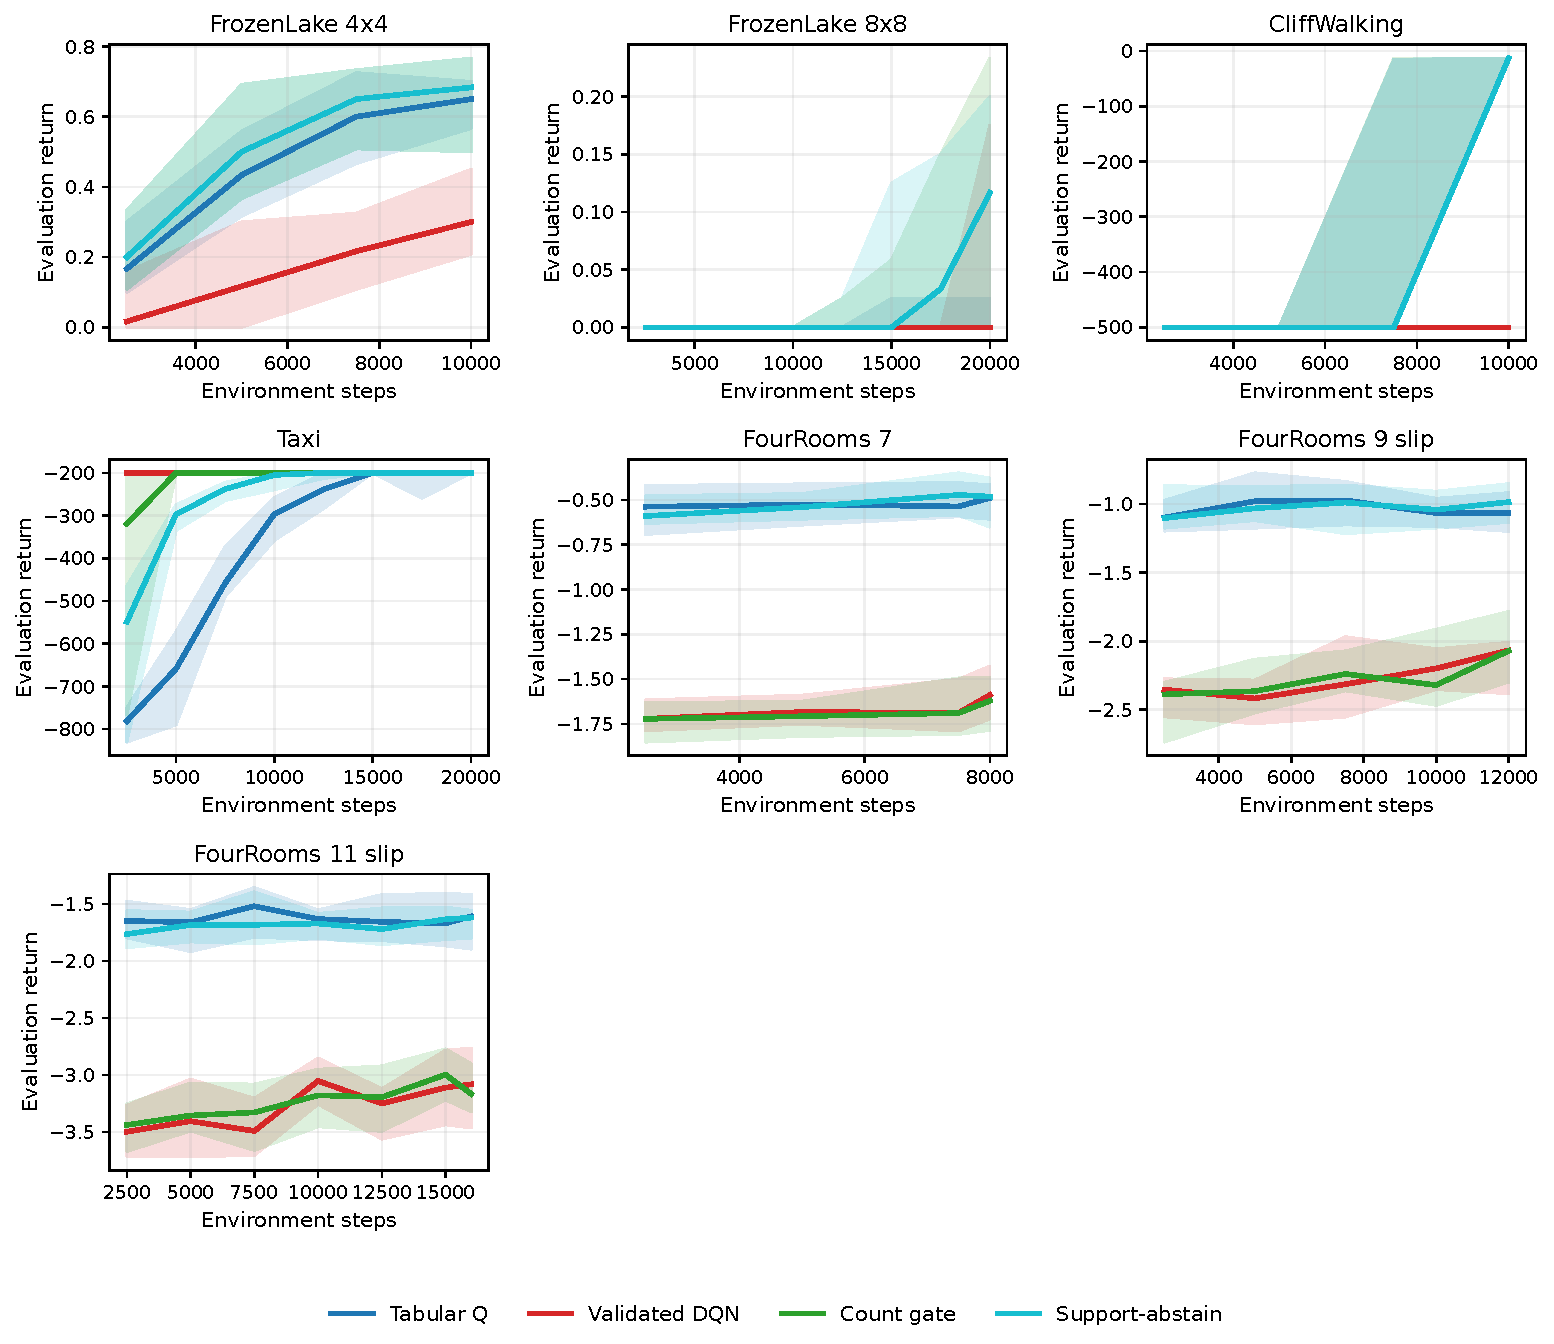
\includegraphics[width=\textwidth]{figures/Figure_01A_Compact_Task_Learning_Curves.pdf}
\caption{Median evaluation-return learning curves and interquartile bands for
the seven compact tasks. Curves use 30 independently seeded runs per method.}
\label{fig:compact-curves}
\end{figure*}

\begin{table*}[t]
\centering
\scriptsize
\caption{Return AUC for core methods in the confirmatory compact expansion.
Intervals are seed-bootstrap 95\% intervals.}
\label{tab:compact-performance}
\resizebox{\textwidth}{!}{\begin{tabular}{llclc}
\toprule
Environment & Method & Seeds & Mean AUC [bootstrap 95\% CI] & Median AUC \\
\midrule
CliffWalking & Count gate & 30 & -356.672 [-386.389, -326.911] & -419 \\
CliffWalking & Support-abstain & 30 & -381.589 [-442.400, -337.811] & -419 \\
CliffWalking & Tabular Q & 30 & -386.363 [-438.387, -340.800] & -419 \\
CliffWalking & Validated DQN & 30 & -500.000 [-500.000, -500.000] & -500 \\
FourRooms 11 slip & Count gate & 30 & -3.233 [-3.295, -3.175] & -3.22 \\
FourRooms 11 slip & Support-abstain & 30 & -1.671 [-1.701, -1.642] & -1.68 \\
FourRooms 11 slip & Tabular Q & 30 & -1.649 [-1.678, -1.618] & -1.65 \\
FourRooms 11 slip & Validated DQN & 30 & -3.297 [-3.344, -3.250] & -3.32 \\
FourRooms 7 & Count gate & 30 & -1.687 [-1.722, -1.652] & -1.69 \\
FourRooms 7 & Support-abstain & 30 & -0.522 [-0.548, -0.495] & -0.527 \\
FourRooms 7 & Tabular Q & 30 & -0.538 [-0.569, -0.507] & -0.537 \\
FourRooms 7 & Validated DQN & 30 & -1.667 [-1.701, -1.633] & -1.67 \\
FourRooms 9 slip & Count gate & 30 & -2.265 [-2.319, -2.210] & -2.25 \\
FourRooms 9 slip & Support-abstain & 30 & -1.022 [-1.053, -0.991] & -1.03 \\
FourRooms 9 slip & Tabular Q & 30 & -1.034 [-1.072, -0.998] & -1.02 \\
FourRooms 9 slip & Validated DQN & 30 & -2.303 [-2.363, -2.241] & -2.32 \\
FrozenLake 4x4 & Count gate & 30 & 0.525 [0.486, 0.562] & 0.556 \\
FrozenLake 4x4 & Support-abstain & 30 & 0.525 [0.486, 0.562] & 0.556 \\
FrozenLake 4x4 & Tabular Q & 30 & 0.494 [0.461, 0.529] & 0.481 \\
FrozenLake 4x4 & Validated DQN & 30 & 0.209 [0.175, 0.244] & 0.189 \\
FrozenLake 8x8 & Count gate & 30 & 0.042 [0.026, 0.060] & 0.0202 \\
FrozenLake 8x8 & Support-abstain & 30 & 0.047 [0.029, 0.068] & 0.0298 \\
FrozenLake 8x8 & Tabular Q & 30 & 0.010 [0.004, 0.019] & 0.00238 \\
FrozenLake 8x8 & Validated DQN & 30 & 0.015 [0.009, 0.022] & 0.00595 \\
Taxi & Count gate & 30 & -224.226 [-236.632, -213.394] & -209 \\
Taxi & Support-abstain & 30 & -259.430 [-266.809, -252.208] & -257 \\
Taxi & Tabular Q & 30 & -378.605 [-392.533, -365.890] & -366 \\
Taxi & Validated DQN & 30 & -212.341 [-225.605, -201.426] & -200 \\
\bottomrule
\end{tabular}
}
\end{table*}

\subsection{RQ2: Does count gating outperform tabular Q-learning?}

No general advantage is supported. Count gating and tabular Q-learning are
not significantly different on CliffWalking or FrozenLake 4x4 after
correction. Count gating improves over tabular learning on Taxi by 154.4
([135.8, 173.0], $t$-Holm $p=1.62\times10^{-14}$), but is substantially
worse on all three held-out-goal FourRooms tasks: mean deficits are 1.149,
1.231, and 1.584, with all 30 pairs favoring tabular learning in each task.
The FrozenLake 8x8 mean gain of 0.032 does not survive the mean-based Holm
family ($p=0.0947$). Across the seven compact tasks, support abstention has the
best mean environment rank (2.07), count gating ranks second (2.93), and
tabular learning ranks third (3.43); these ranks are descriptive and do not
imply a common-scale performance effect.

\subsection{RQ3: What happens under held-out exact-state support shift?}

In FourRooms, changing the goal changes the exact state key while preserving a
structured coordinate input for the network. Count gating, fixed mixing, and
the validated DQN all obtain strongly negative AUCs. Tabular and random
tie-breaking are much less negative. This pattern is consistent across sizes
7, 9, and 11: low or zero support increases reliance on neural extrapolation,
but that extrapolation is not reliable. Figure~\ref{fig:support-boundary}
links the empirical result to the gate definition.

\begin{figure*}[t]
\centering
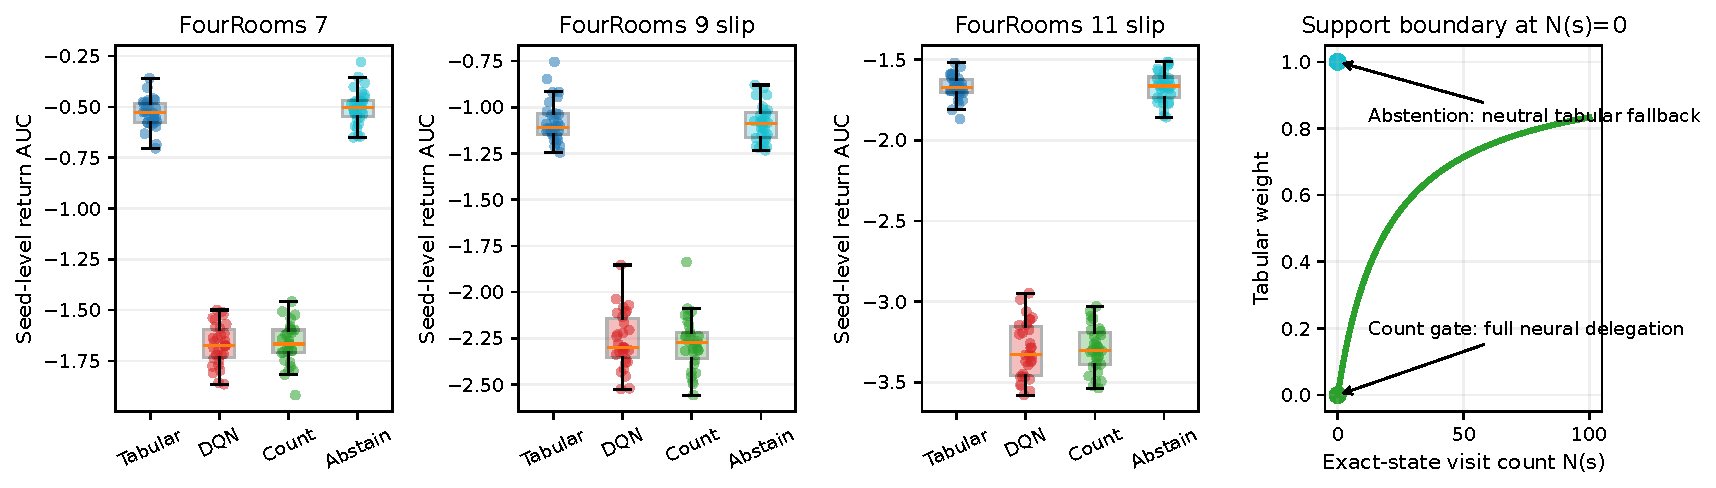
\includegraphics[width=\textwidth]{figures/Figure_02_Support_Boundary_and_Abstention_Replication.pdf}
\caption{Support boundary and neural extrapolation failure. The first three
panels show the independently seeded replication. The final panel shows why
the standard count gate delegates completely to the neural estimator at
$N(s)=0$, whereas support abstention uses a neutral fallback.}
\label{fig:support-boundary}
\end{figure*}

\subsection{RQ4: Does support abstention replicate the specific repair?}

Yes for the discovered FourRooms mechanism, not universally.
Table~\ref{tab:support-replication} uses new seeds 300--329. Support abstention
improves over count gating by 1.164 on FourRooms 7
([1.117, 1.211]), 1.190 on FourRooms 9
([1.142, 1.238]), and 1.625 on FourRooms 11
([1.560, 1.689]). All 30 pairs favor abstention in every environment;
mean-based Holm values are below $8.0\times10^{-28}$ and
Wilcoxon-Holm values are $3.73\times10^{-8}$. Support abstention is not
superior to tabular learning after correction on these tasks, which indicates
repair of harmful extrapolation rather than new transfer.

On the independent MiniGrid Empty-5x5 replication, abstention and count gating
are not different (mean difference 0.019, interval [$-0.034$, 0.070],
$t$-Holm $p=1$). This neutral replication is important: support abstention is
a boundary-specific repair, not a universal improvement.

\begin{table*}[t]
\centering
\small
\caption{Support-abstention versus count-gating replication after diagnostic
discovery. Positive differences favor abstention.}
\label{tab:support-replication}
\resizebox{\textwidth}{!}{\begin{tabular}{lclccc}
\toprule
Environment & Pairs & Mean difference [bootstrap 95\% CI] & t-Holm p & Wilcoxon-Holm p & Wins/losses/ties \\
\midrule
FourRooms 11 slip held-out & 30 & 1.625 [1.560, 1.689] & 4.54e-28 & 3.73e-08 & 30/0/0 \\
FourRooms 7 held-out & 30 & 1.164 [1.117, 1.211] & 6.06e-28 & 3.73e-08 & 30/0/0 \\
FourRooms 9 slip held-out & 30 & 1.190 [1.142, 1.238] & 7.98e-28 & 3.73e-08 & 30/0/0 \\
MiniGrid Empty 5x5 & 30 & 0.019 [-0.034, 0.070] & 1 & 1 & 7/4/19 \\
\bottomrule
\end{tabular}
}
\end{table*}

\subsection{RQ5: Are conclusions robust to DQN tuning and task expansion?}

The development-only sweep selects the vanilla 128-unit DQN with learning rate
$3\times10^{-4}$, replay capacity 100,000, warm-up 512, and target interval
500. The Double-DQN candidate is not selected. In independent validation, the
selected configuration has a better descriptive mean environment rank than
the original comparator (1.25 versus 1.75), but no per-environment planned
contrast survives Holm correction. FrozenLake 4x4 and 8x8 have positive
uncorrected bootstrap intervals, while Taxi includes a large negative tail.
Accordingly, the comparator is more extensively validated, but the study does
not claim a statistically established universal DQN improvement.

\begin{figure*}[t]
\centering
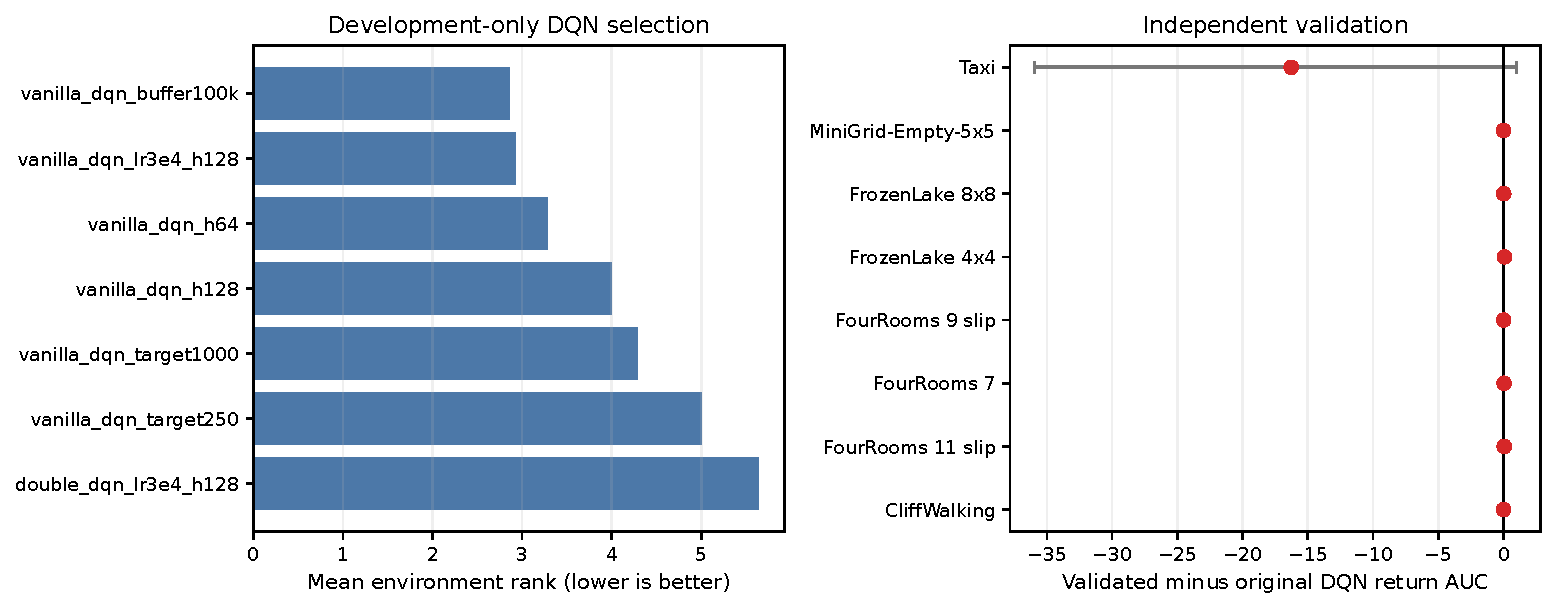
\includegraphics[width=\textwidth]{figures/Figure_03_DQN_Comparator_Selection_and_Validation.pdf}
\caption{DQN development selection and independent validation. Lower
development rank is better. Validation differences are selected minus
original DQN AUC with bootstrap 95\% intervals.}
\label{fig:dqn-validation}
\end{figure*}

\begin{table*}[t]
\centering
\small
\caption{Independent validation of the development-selected DQN. Positive
differences favor the validated configuration.}
\label{tab:dqn-validation}
\resizebox{\textwidth}{!}{\begin{tabular}{lclcc}
\toprule
Environment & Pairs & Mean difference [bootstrap 95\% CI] & t-Holm p & Wins/losses/ties \\
\midrule
CliffWalking & 30 & 0.000 [0.000, 0.000] & 1 & 0/0/30 \\
FourRooms 11 slip & 30 & 0.053 [-0.028, 0.136] & 0.91 & 16/14/0 \\
FourRooms 7 & 30 & 0.038 [-0.009, 0.086] & 0.667 & 18/12/0 \\
FourRooms 9 slip & 30 & 0.009 [-0.054, 0.072] & 1 & 16/14/0 \\
FrozenLake 4x4 & 30 & 0.071 [0.011, 0.131] & 0.232 & 20/9/1 \\
FrozenLake 8x8 & 30 & 0.011 [0.002, 0.021] & 0.232 & 16/9/5 \\
MiniGrid Empty 5x5 & 10 & 0.000 [0.000, 0.000] & 1 & 0/0/10 \\
Taxi & 30 & -16.273 [-35.978, 1.003] & 0.626 & 1/6/23 \\
\bottomrule
\end{tabular}
}
\end{table*}

Expanded MiniGrid evidence is heterogeneous
(Fig.~\ref{fig:minigrid-curves}, Table~\ref{tab:minigrid}). Count gating
improves over the validated DQN after Holm correction only on Empty 8x8
(difference 0.596, interval [0.442, 0.750], $p=0.000761$). The validated DQN
has zero AUC on several layouts. Tabular Q-learning has the best descriptive
mean environment rank (1.58) and substantially exceeds count gating on both
DoorKey tasks and Empty 8x8 in raw means, although not every comparison
survives the configured family correction. MiniGrid FourRooms shows a small
abstention-over-count difference of 0.012, with all ten pairs favoring
abstention. These results broaden the failure evidence but do not establish a
single best method.

\begin{figure*}[t]
\centering
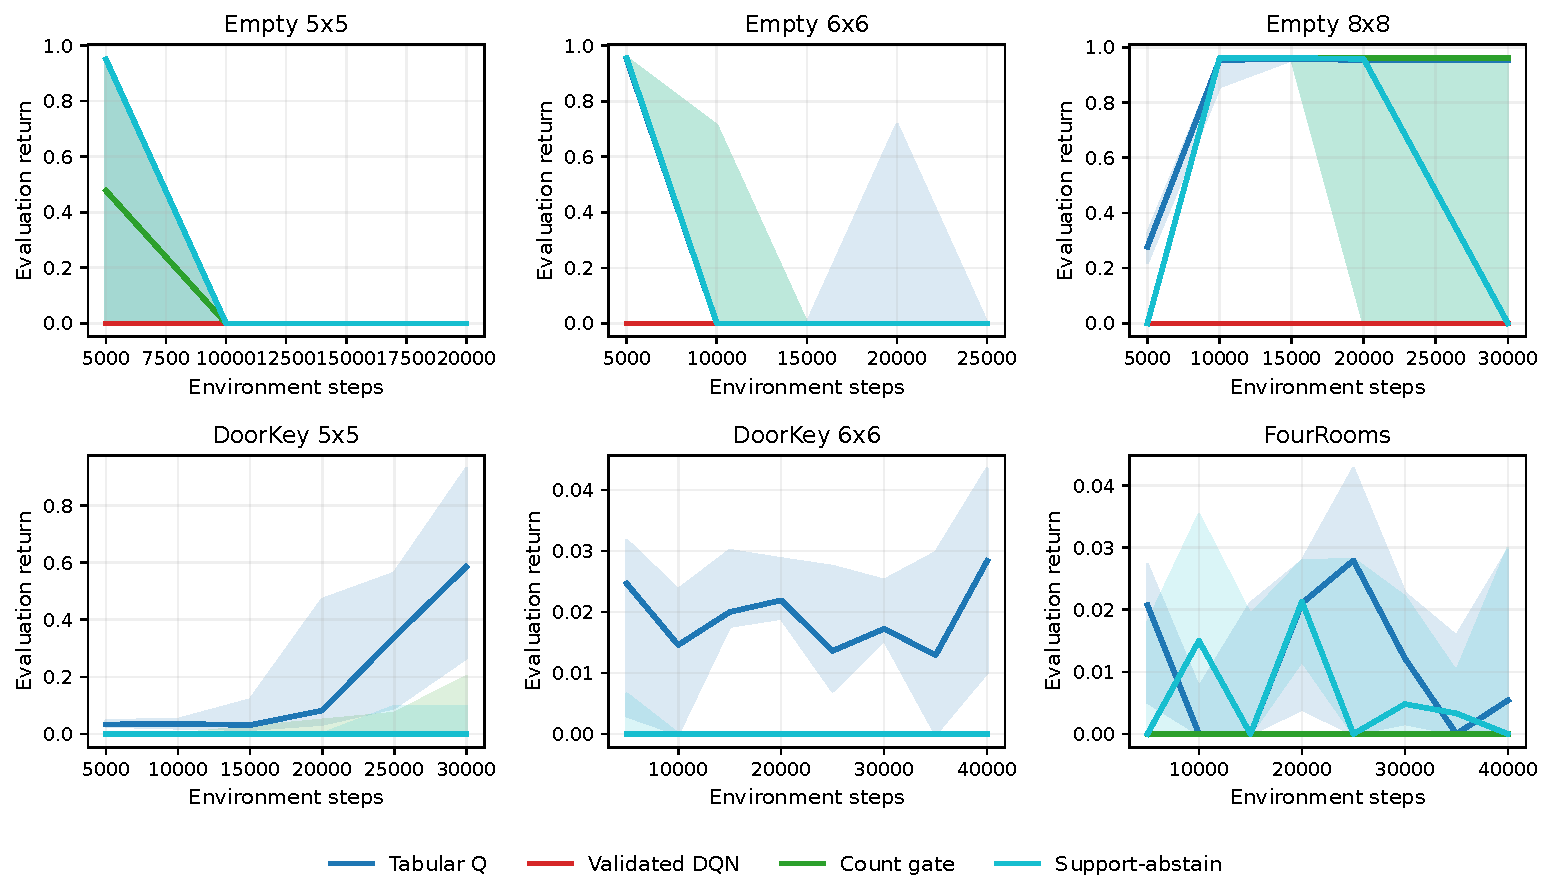
\includegraphics[width=\textwidth]{figures/Figure_04_MiniGrid_Diagnostic_Learning_Curves.pdf}
\caption{Median learning curves and interquartile bands for the six fully
observable MiniGrid diagnostics, ten seeds per method.}
\label{fig:minigrid-curves}
\end{figure*}

\begin{table*}[t]
\centering
\scriptsize
\caption{Return AUC in the extended MiniGrid diagnostic. This family is post
hoc and uses ten seeds; it is not pooled with compact confirmation.}
\label{tab:minigrid}
\resizebox{\textwidth}{!}{\begin{tabular}{llclc}
\toprule
Environment & Method & Seeds & Mean AUC [bootstrap 95\% CI] & Median AUC \\
\midrule
DoorKey 5x5 & Count gate & 10 & 0.041 [0.001, 0.083] & 0 \\
DoorKey 5x5 & Support-abstain & 10 & 0.033 [0.000, 0.080] & 0 \\
DoorKey 5x5 & Tabular Q & 10 & 0.210 [0.116, 0.309] & 0.147 \\
DoorKey 5x5 & Validated DQN & 10 & 0.000 [0.000, 0.000] & 0 \\
DoorKey 6x6 & Count gate & 10 & 0.000 [0.000, 0.000] & 0 \\
DoorKey 6x6 & Support-abstain & 10 & 0.000 [0.000, 0.001] & 0 \\
DoorKey 6x6 & Tabular Q & 10 & 0.021 [0.017, 0.026] & 0.0189 \\
DoorKey 6x6 & Validated DQN & 10 & 0.000 [0.000, 0.000] & 0 \\
Empty 5x5 & Count gate & 10 & 0.159 [0.064, 0.254] & 0.159 \\
Empty 5x5 & Support-abstain & 10 & 0.175 [0.094, 0.270] & 0.159 \\
Empty 5x5 & Tabular Q & 10 & 0.190 [0.079, 0.317] & 0.158 \\
Empty 5x5 & Validated DQN & 10 & 0.000 [0.000, 0.000] & 0 \\
Empty 6x6 & Count gate & 10 & 0.203 [0.107, 0.310] & 0.12 \\
Empty 6x6 & Support-abstain & 10 & 0.262 [0.167, 0.381] & 0.12 \\
Empty 6x6 & Tabular Q & 10 & 0.214 [0.143, 0.298] & 0.12 \\
Empty 6x6 & Validated DQN & 10 & 0.000 [0.000, 0.000] & 0 \\
Empty 8x8 & Count gate & 10 & 0.596 [0.442, 0.750] & 0.577 \\
Empty 8x8 & Support-abstain & 10 & 0.586 [0.452, 0.720] & 0.577 \\
Empty 8x8 & Tabular Q & 10 & 0.779 [0.652, 0.876] & 0.865 \\
Empty 8x8 & Validated DQN & 10 & 0.000 [0.000, 0.000] & 0 \\
FourRooms & Count gate & 10 & 0.002 [0.000, 0.003] & 0 \\
FourRooms & Support-abstain & 10 & 0.014 [0.012, 0.016] & 0.0133 \\
FourRooms & Tabular Q & 10 & 0.017 [0.012, 0.021] & 0.02 \\
FourRooms & Validated DQN & 10 & 0.002 [0.000, 0.003] & 0 \\
\bottomrule
\end{tabular}
}
\end{table*}

\subsection{RQ6: What does the application-oriented support shift show?}

The application study completed all 180 planned runs and passed the result
audit. Figure~\ref{fig:application-case} and
Table~\ref{tab:application-case} show the central trade-off. Evaluation states
are unsupported on approximately 39.2\% of decision steps for every method.
The fuzzy gate improves AUC over the validated DQN by 0.575
([0.152, 0.987], $t$-Holm $p=0.0256$, Wilcoxon-Holm $p=0.0163$), but its
0.211 difference from count gating is not significant
([$-0.171$, 0.626]). It remains worse than support abstention by 2.520 and
tabular Q-learning by 2.299; 29 of 30 paired seeds favor each comparator.

The outcome metrics explain why a single performance number is insufficient.
Tabular Q-learning has the highest final success rate (0.751), while support
abstention has lower success (0.544) but only 0.007 collision rate because its
unsupported-state decision is the hold action. Fuzzy arbitration reaches
0.498 success but has 0.244 collision rate. These results support a
decision-support interpretation: a safe fallback can reduce harmful motion
without creating transfer, whereas neural fallback can improve some learning
comparisons while retaining deployment risk.

\begin{figure*}[t]
\centering
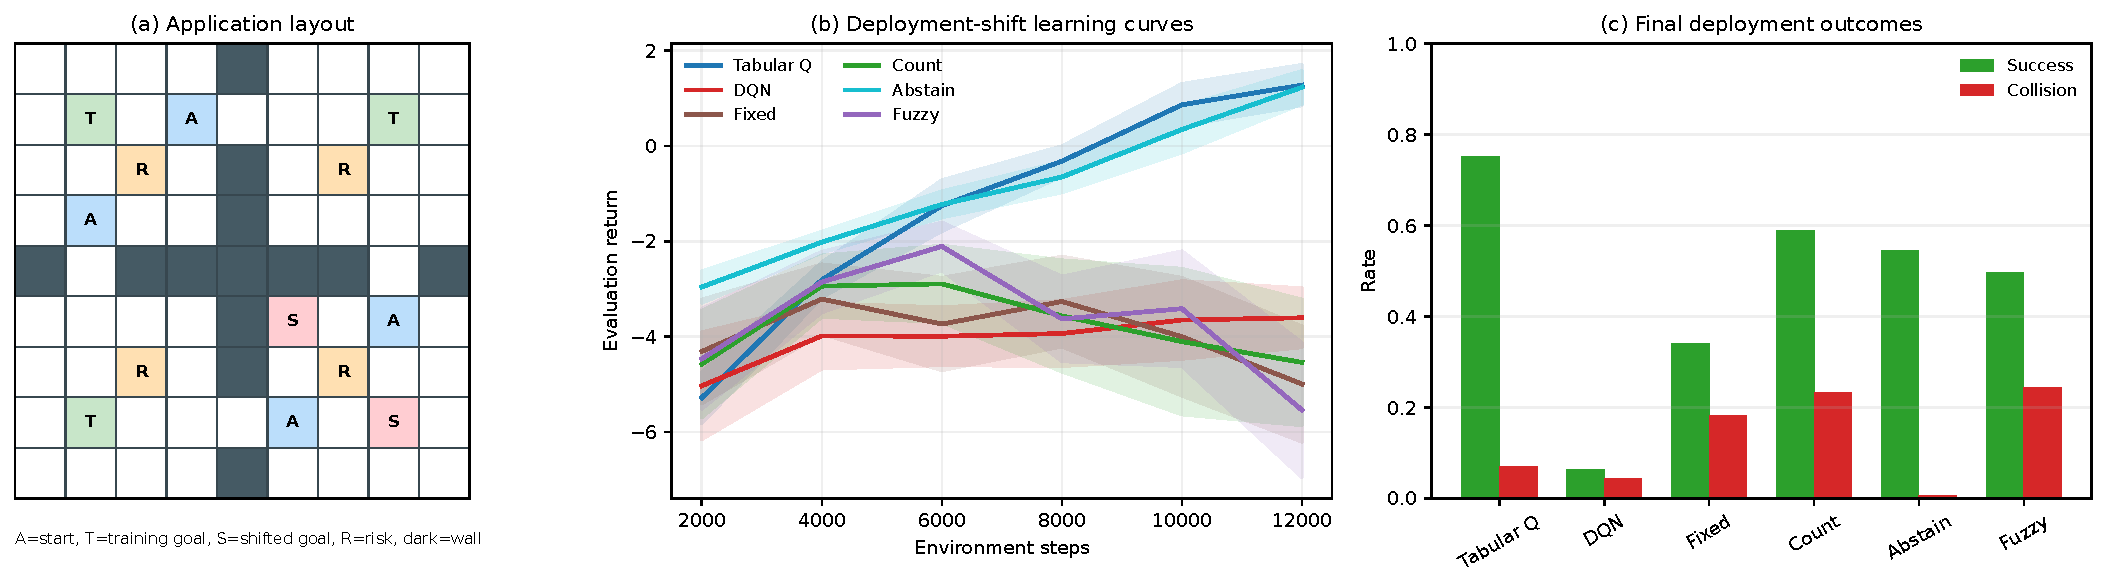
\includegraphics[width=\textwidth]{figures/Figure_05_Application_Case_Study.pdf}
\caption{Application-inspired navigation under deployment goal shift. Panel
(a) shows the controlled map: starts, recurring training goals, shifted
deployment goals, risk cells, and walls. Panels (b) and (c) report learning
curves and final deployment outcomes.}
\label{fig:application-case}
\end{figure*}

\begin{table*}[t]
\centering
\scriptsize
\caption{Application-navigation outcomes at deployment shift. Rates are
seed means; AUC intervals are seed-bootstrap 95\% intervals.}
\label{tab:application-case}
\resizebox{\textwidth}{!}{\begin{tabular}{lcccccc}
\toprule
Method & Return AUC [95\% bootstrap CI] & Success & Failure & Collision & Unsupported & Abstention \\
\midrule
Count gate & -3.612 [-4.201, -3.043] & 0.590 & 0.410 & 0.233 & 0.392 & 0.000 \\
Fixed mixture & -3.773 [-4.490, -3.113] & 0.341 & 0.659 & 0.183 & 0.393 & 0.000 \\
Fuzzy adaptive & -3.401 [-3.861, -2.978] & 0.498 & 0.502 & 0.244 & 0.393 & 0.000 \\
Support abstention & -0.881 [-1.108, -0.649] & 0.544 & 0.456 & 0.007 & 0.392 & 0.392 \\
Tabular Q & -1.102 [-1.326, -0.891] & 0.751 & 0.249 & 0.070 & 0.392 & 0.392 \\
Validated DQN & -3.976 [-4.345, -3.630] & 0.064 & 0.936 & 0.044 & 0.393 & 0.000 \\
\bottomrule
\end{tabular}
}
\end{table*}

\subsection{RQ7: Does fuzzy arbitration generalize, and what does it cost?}

Table~\ref{tab:adaptive-gate} reports the independently seeded compact
validation. Relative to DQN, fuzzy arbitration improves FrozenLake 4x4 AUC by
0.291 ([0.244, 0.338], $t$-Holm $p=1.12\times10^{-11}$), with all 30 seeds
favoring the fuzzy method. On CliffWalking the mean difference is 925 with a
positive bootstrap interval, but heavy tails leave the mean-based Holm test
nonsignificant; the Wilcoxon-Holm sensitivity test is $p=1.45\times10^{-4}$.
The fuzzy gate does not significantly beat count gating in any of the three
tasks. Under complete FourRooms support shift, its mean alpha is zero, so it
matches neural fallback and is worse than both tabular and support-abstention
methods in all 30 paired seeds.

\begin{table*}[t]
\centering
\small
\caption{Return AUC in the 30-seed fuzzy adaptive-gate validation.}
\label{tab:adaptive-gate}
\resizebox{\textwidth}{!}{\begin{tabular}{lll}
\toprule
Environment & Method & Return AUC [95\% bootstrap CI] \\
\midrule
CliffWalking & Count gate & -491.575 [-598.365, -400.000] \\
CliffWalking & Fuzzy adaptive & -400.017 [-467.333, -346.083] \\
CliffWalking & Support abstention & -412.547 [-488.410, -354.271] \\
CliffWalking & Tabular Q & -474.701 [-558.106, -401.679] \\
CliffWalking & Validated DQN & -1325.000 [-2150.000, -706.250] \\
FourRooms 9 support shift & Count gate & -2.280 [-2.323, -2.240] \\
FourRooms 9 support shift & Fuzzy adaptive & -2.280 [-2.329, -2.231] \\
FourRooms 9 support shift & Support abstention & -1.084 [-1.108, -1.062] \\
FourRooms 9 support shift & Tabular Q & -1.085 [-1.119, -1.053] \\
FourRooms 9 support shift & Validated DQN & -2.279 [-2.324, -2.234] \\
FrozenLake 4x4 & Count gate & 0.528 [0.498, 0.558] \\
FrozenLake 4x4 & Fuzzy adaptive & 0.505 [0.472, 0.538] \\
FrozenLake 4x4 & Support abstention & 0.524 [0.495, 0.553] \\
FrozenLake 4x4 & Tabular Q & 0.450 [0.412, 0.487] \\
FrozenLake 4x4 & Validated DQN & 0.214 [0.179, 0.253] \\
\bottomrule
\end{tabular}
}
\end{table*}

Figure~\ref{fig:fuzzy-sensitivity} adds a direct decision-surface sensitivity
analysis for the fuzzy gate. It varies $\tau_N$, $\kappa$, membership shape,
consequents, and the explicit zero-support rule without retraining an RL
agent. The important boundary remains invariant: at $N(s)=0$, the configured
neural-fallback fuzzy gate assigns zero memory weight. Lower $\tau_N$ moves
the gate toward memory after fewer visits, higher $\tau_N$ delays memory use,
and $\kappa$ changes how rapidly TD-error evidence is treated as neural
uncertainty. This analysis justifies the fuzzy surface as an interpretable
ablation target rather than a hidden constant.

\begin{figure*}[t]
\centering
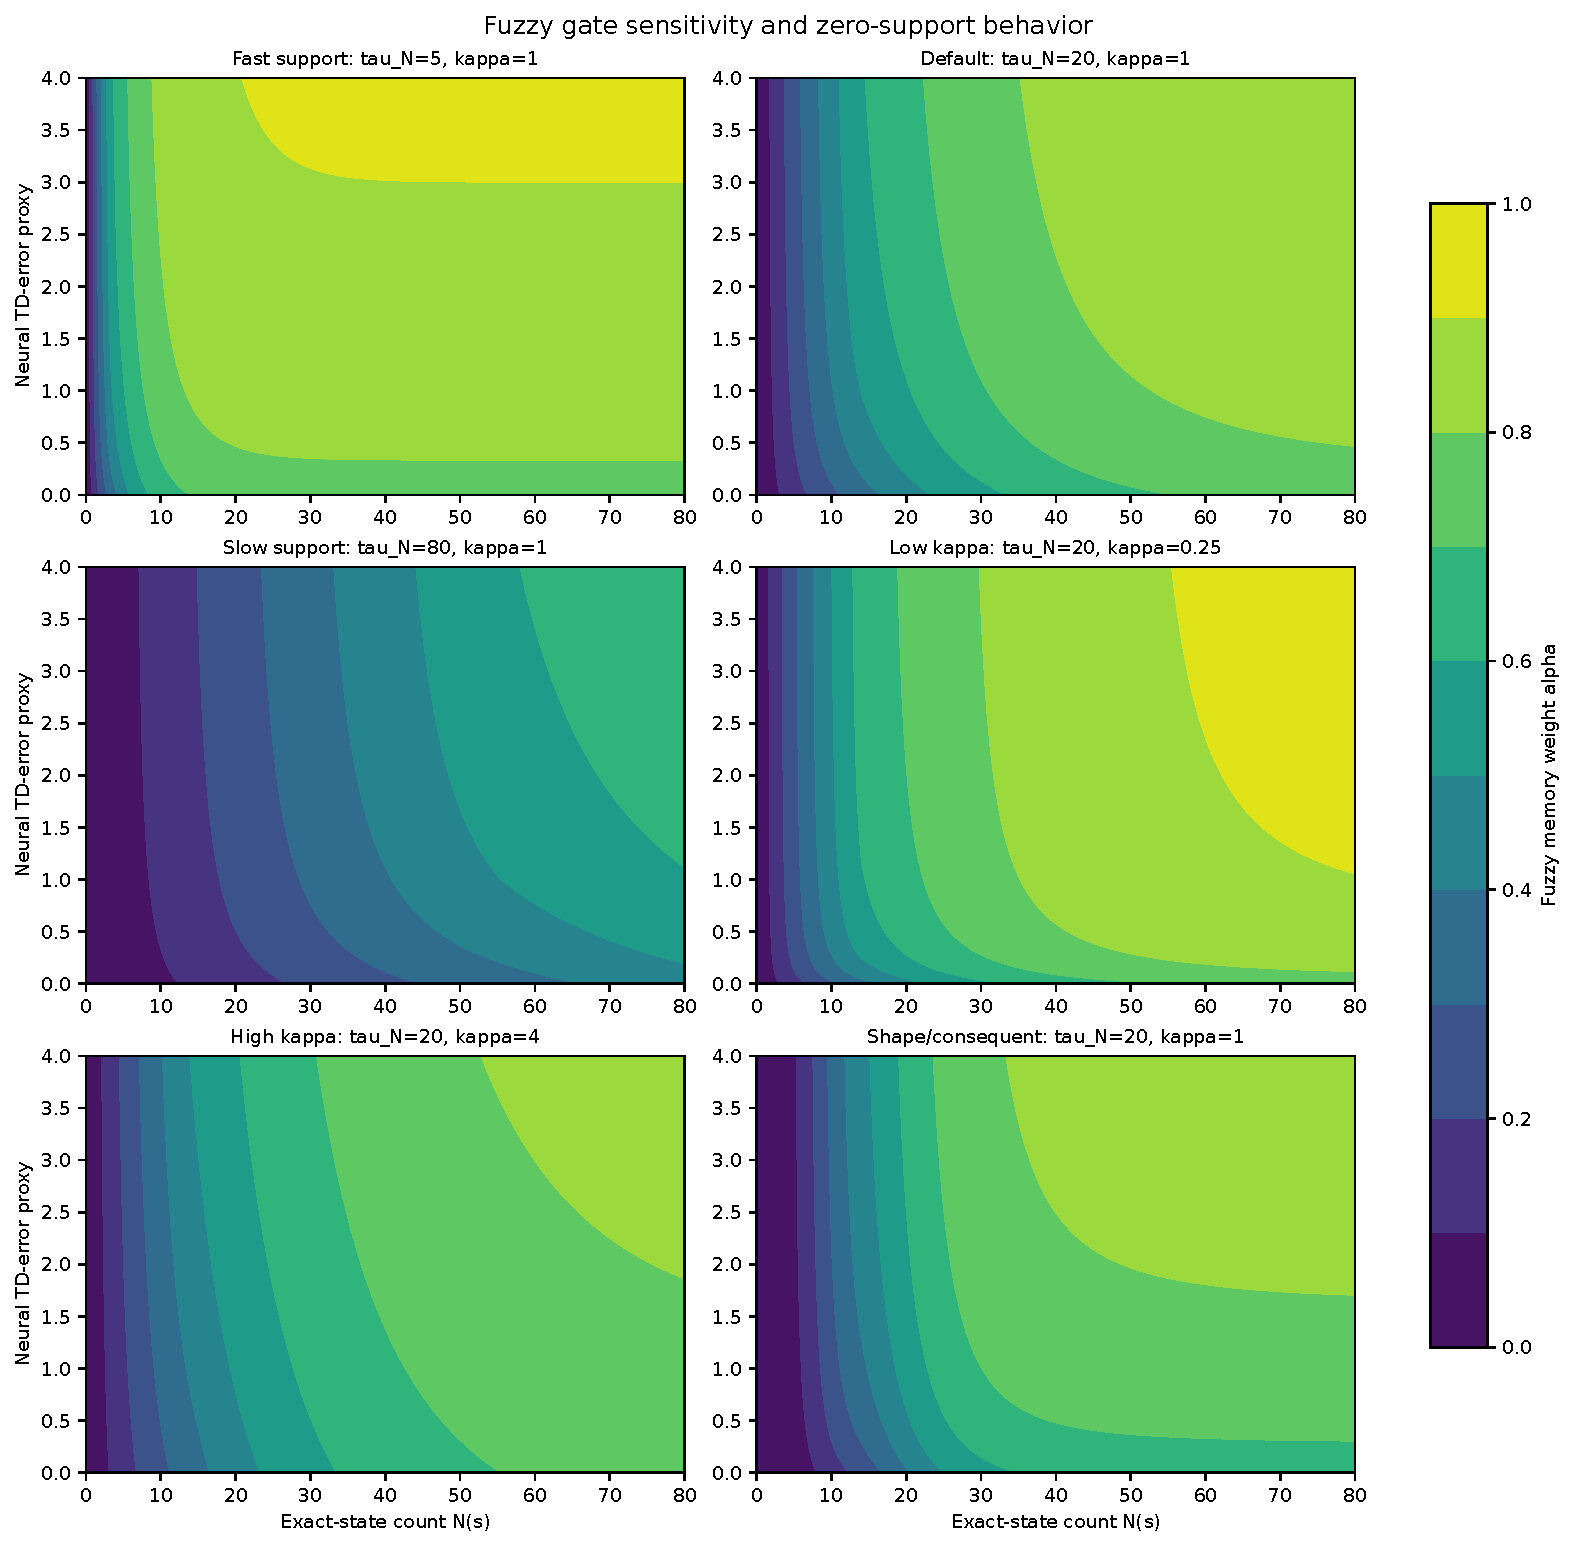
\includegraphics[width=\textwidth]{figures/Figure_06_Fuzzy_Gate_Sensitivity.pdf}
\caption{Analytic fuzzy-gate sensitivity to $\tau_N$, $\kappa$, membership
shape, consequents, and zero-support behavior. The vertical zero-count boundary
shows the explicit neural-fallback setting used in the reported fuzzy baseline.}
\label{fig:fuzzy-sensitivity}
\end{figure*}

The ten-seed descriptive cost family in
Table~\ref{tab:cost-support} and Figure~\ref{fig:cost-support} shows that fuzzy
logic is not free. In application navigation, mean decision times are
134~$\mu$s for tabular Q-learning, 349~$\mu$s for support abstention,
442~$\mu$s for DQN, 573~$\mu$s for count gating, and 713~$\mu$s for fuzzy
arbitration. FourRooms shows the same ordering between count and fuzzy gates
(485 versus 655~$\mu$s). Exact-memory lower-bound estimates are about
5.4~KiB in application navigation and 32.8~KiB for fuzzy arbitration in
FourRooms; the DQN's zero denotes no exact-state table, not zero neural-model
memory. Timings are machine- and contention-dependent descriptive
measurements, not hardware-independent complexity claims.

\begin{table*}[t]
\centering
\scriptsize
\caption{Support, branch use, exact-memory lower bound, and decision time.
The DQN exact-memory fields are zero because neural parameters are excluded.}
\label{tab:cost-support}
\resizebox{\textwidth}{!}{\begin{tabular}{llccccccc}
\toprule
Environment & Method & Unsupported & Memory branch & Neural branch & Abstention & Stored states & Estimated KiB & Decision time (us) \\
\midrule
Application navigation & Count gate & 0.430 & 0.437 & 0.563 & 0.000 & 198.5 & 5.43 & 573.3 \\
Application navigation & Fuzzy adaptive & 0.430 & 0.432 & 0.568 & 0.000 & 196.8 & 5.38 & 713.1 \\
Application navigation & Support abstention & 0.430 & 0.439 & 0.131 & 0.430 & 197.6 & 5.40 & 348.5 \\
Application navigation & Tabular Q & 0.430 & 0.570 & 0.000 & 0.430 & 199.0 & 5.44 & 134.1 \\
Application navigation & Validated DQN & 0.430 & 0.000 & 1.000 & 0.000 & 0.0 & 0.00 & 442.5 \\
FourRooms 9 support shift & Count gate & 1.000 & 0.000 & 1.000 & 0.000 & 1401.7 & 32.85 & 485.0 \\
FourRooms 9 support shift & Fuzzy adaptive & 1.000 & 0.000 & 1.000 & 0.000 & 1401.1 & 32.84 & 655.1 \\
FourRooms 9 support shift & Support abstention & 1.000 & 0.000 & 0.000 & 1.000 & 1524.3 & 35.73 & 168.9 \\
FourRooms 9 support shift & Tabular Q & 1.000 & 0.000 & 0.000 & 1.000 & 1903.6 & 44.62 & 132.4 \\
FourRooms 9 support shift & Validated DQN & 1.000 & 0.000 & 1.000 & 0.000 & 0.0 & 0.00 & 416.8 \\
\bottomrule
\end{tabular}
}
\end{table*}

\begin{figure*}[t]
\centering
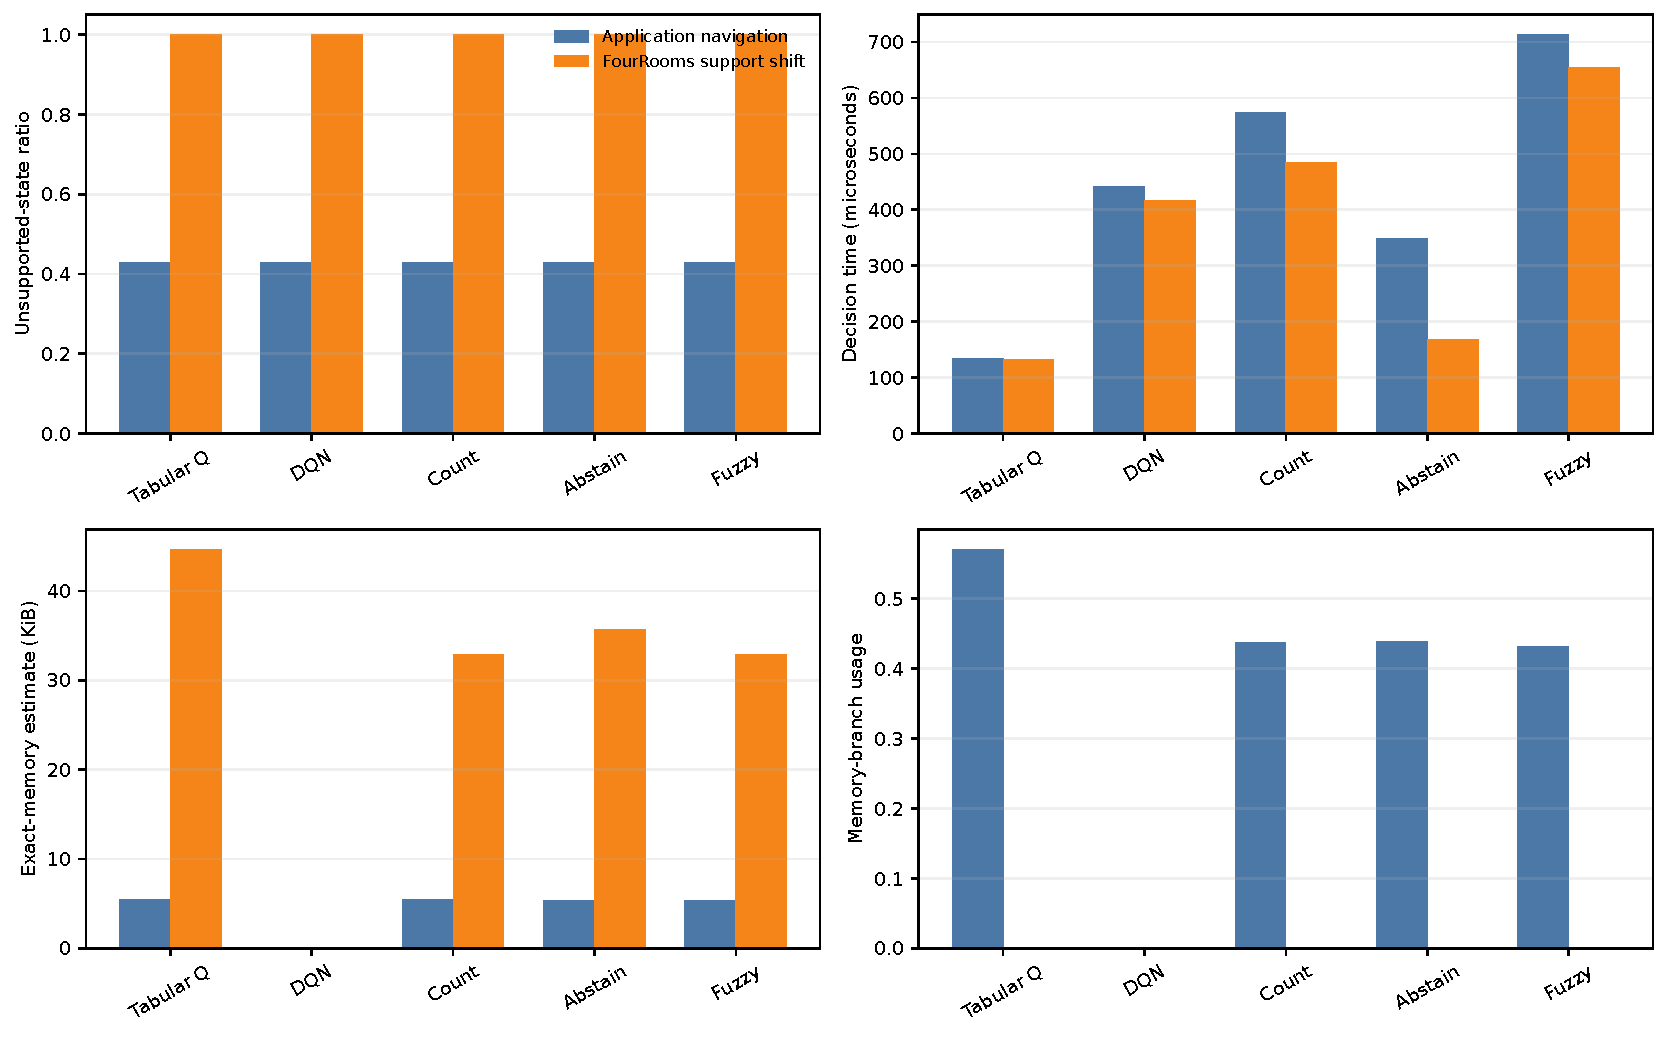
\includegraphics[width=\textwidth]{figures/Figure_07_Cost_Support_and_Unsupported_Ratio.pdf}
\caption{Descriptive cost and support metrics in the ten-seed analysis.
Decision timers exclude environment stepping; memory is the documented
exact-table lower bound.}
\label{fig:cost-support}
\end{figure*}

Figure~\ref{fig:extended-ranks} summarizes the task-specific ranks. It makes
the central boundary visible: count gating is competitive on recurrent tasks
with a weak neural comparator, abstention protects held-out support, and
tabular learning remains difficult to beat in compact discrete domains.

\begin{figure}[t]
\centering
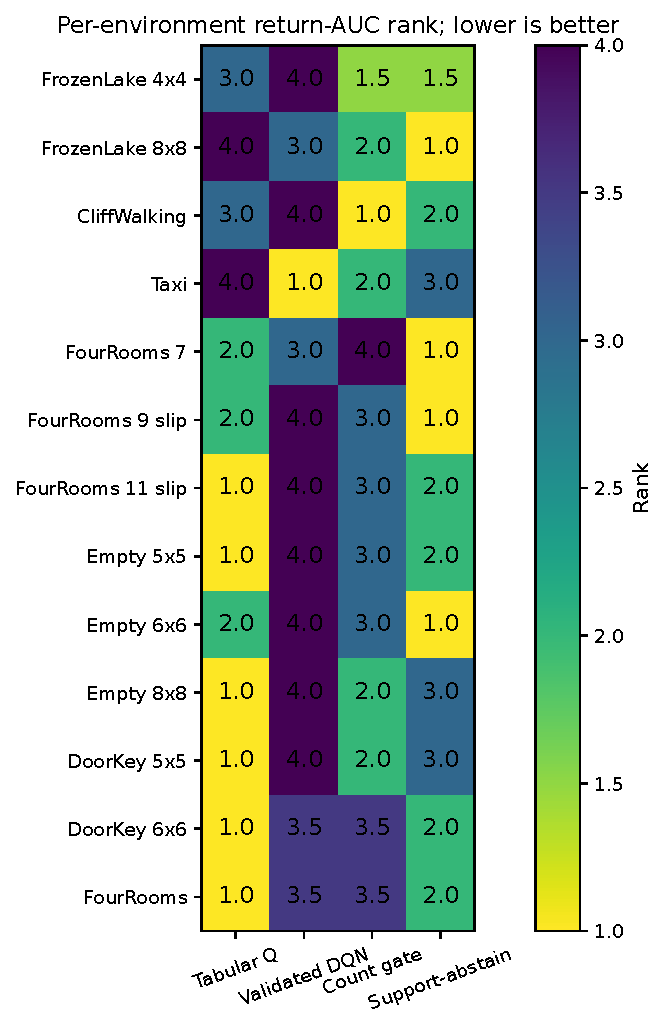
\includegraphics[width=0.80\linewidth]{figures/Figure_08_Compact_and_MiniGrid_Rank_Summary.pdf}
\caption{Per-environment return-AUC ranks across the compact expansion and
extended MiniGrid diagnostic. Lower is better; ranks are descriptive because
raw returns are not commensurate across tasks.}
\label{fig:extended-ranks}
\end{figure}
\FloatBarrier


\begin{table*}[t]
\centering
\scriptsize
\caption{Audited dependency-free smoke validations added for revision-risk checks. These small runs verify executable approximate-support, fuzzy-ablation, and stronger-baseline code paths; they are not used as full confirmatory performance evidence.}
\label{tab:addon-smoke-validation}
\resizebox{\textwidth}{!}{\begin{tabular}{lllrl}
\toprule
Validation family & Environment & Method & Seeds & Return AUC \\
\midrule
Approximate support smoke & Application navigation & approx\_count\_gated\_k5 & 3 & -5.835 [-13.932, -1.653] \\
Approximate support smoke & Application navigation & count\_gated\_tau\_20 & 3 & -6.040 [-14.545, -1.653] \\
Approximate support smoke & Application navigation & support\_abstain\_tau\_20 & 3 & -1.786 [-1.922, -1.653] \\
Approximate support smoke & Application navigation & tabular & 3 & -2.900 [-4.698, -0.656] \\
Fuzzy ablation smoke & Application navigation & fuzzy\_kappa\_025 & 2 & -2.575 [-2.985, -2.165] \\
Fuzzy ablation smoke & Application navigation & fuzzy\_kappa\_4 & 2 & -2.575 [-2.985, -2.165] \\
Fuzzy ablation smoke & Application navigation & fuzzy\_shoulder\_conservative & 2 & -2.575 [-2.985, -2.165] \\
Fuzzy ablation smoke & Application navigation & fuzzy\_tau\_20 & 2 & -2.575 [-2.985, -2.165] \\
Fuzzy ablation smoke & Application navigation & fuzzy\_tau\_5 & 2 & -2.575 [-2.985, -2.165] \\
Fuzzy ablation smoke & Application navigation & fuzzy\_tau\_80 & 2 & -2.575 [-2.985, -2.165] \\
Fuzzy ablation smoke & Application navigation & fuzzy\_zero\_support\_abstain & 2 & -0.829 [-0.858, -0.800] \\
Stronger baseline smoke & Application navigation & a2c\_actor\_critic & 2 & -6.981 [-7.068, -6.895] \\
Stronger baseline smoke & Application navigation & dueling\_double\_dqn & 2 & -8.764 [-9.023, -8.505] \\
Stronger baseline smoke & Application navigation & validated\_dqn & 2 & -4.325 [-9.023, 0.373] \\
Stronger baseline smoke & FourRooms 7 & a2c\_actor\_critic & 2 & -0.519 [-0.693, -0.345] \\
Stronger baseline smoke & FourRooms 7 & dueling\_double\_dqn & 2 & -0.789 [-0.790, -0.788] \\
Stronger baseline smoke & FourRooms 7 & validated\_dqn & 2 & -0.520 [-0.695, -0.345] \\
\bottomrule
\end{tabular}
}
\end{table*}

\section{Discussion}
\label{sec:discussion}

The evidence supports a narrow engineering interpretation. Count gating is a
fallback for recurring exact states. When the neural estimator is weak and
the table repeatedly observes the same keys, increasing tabular weight can
improve learning relative to DQN. This occurs on both FrozenLake sizes and
CliffWalking. It does not imply that the hybrid has learned a better general
representation.

Exact-state memory is not a generalization mechanism. Held-out goals remove
table support, and the standard count gate responds by placing more weight on
the neural estimator. The three-size replication shows that this design can
be systematically harmful. Support abstention repairs the particular failure
because it refuses unsupported neural preferences, but it does not create
positive transfer and does not generally exceed tabular learning.

Fuzzy arbitration provides a more graded mechanism but not a different
support boundary. When counts recur, its support and TD-residual inputs can
improve a weak DQN, as observed on FrozenLake 4x4 and in the application AUC
comparison. It does not significantly improve over the simpler count gate.
When support is exactly zero, the configured fuzzy baseline assigns zero
memory weight and inherits the neural branch's extrapolation behavior. Soft
rules should therefore not be interpreted as calibrated confidence or a
safety guarantee merely because they are continuous and interpretable.

The application case makes the engineering trade-off concrete. A hold fallback
nearly removes collisions at unsupported states but sacrifices some final
success relative to tabular learning. Fuzzy and count gates continue to move,
which can improve learning relative to DQN but can also raise collision
exposure. An operator-facing system could use the logged support signal to
request evidence, hand control to a verified planner, or hold position. The
present experiment measures that decision boundary; it does not validate any
particular operational fallback.

Strong tabular baselines materially limit practical advantage in these small
discrete tasks. Taxi is an exception in which count gating improves over
tabular learning while the validated DQN remains competitive. MiniGrid is
mixed: count gating helps relative to the tested DQN on Empty 8x8, but tabular
learning has the best overall rank. The results should therefore be interpreted
as a mechanism and evaluation study, not as evidence that exact-state memory
should be added to arbitrary deep-RL systems.

DQN sensitivity remains a major caveat. The broader development sweep and
independent validation are stronger than a single hand-selected baseline, yet
the selected configuration does not significantly improve every task and
fails on several MiniGrid layouts. More capable architectures, convolutional
representations, longer budgets, and environment-specific tuning could change
the magnitude of hybrid-versus-neural differences. The claim is explicitly
about the tested, audited comparator family.

\section{Limitations}
\label{sec:limitations}

The study uses compact simulated benchmarks, discrete observations or
explicitly encoded discrete images, and limited MiniGrid scale. It includes no
continuous-control task, pixel-based partial observability, real deployment,
or safety-critical intervention. The MiniGrid network is an MLP over a fully
observable flattened image rather than a convolutional architecture.
The application environment is intentionally controlled and does not model
sensor noise, moving obstacles, localization error, actuator dynamics, human
handover, or physical consequences. Its collision and risk metrics must not be
read as field-safety evidence.

The DQN comparator is sensitive to hyperparameters and compute budget. The
development sweep is broader than the original selection but remains finite.
The revised code now includes dueling-DQN and A2C agents and an audited
smoke-validation result family. Because that family is intentionally small and
runs in the dependency-free fallback environment, it verifies executability but
does not support broad performance claims about stronger neural baselines.
The support-abstention idea was discovered after observing the original
FourRooms failure; the new independent seeds support the repair, but the
sequence must remain visible. The MiniGrid expansion is diagnostic and uses
ten seeds per task. Some returns are heavy-tailed, particularly on
CliffWalking, FrozenLake 8x8, and Taxi, so mean and rank-based conclusions can
differ.

Exact-state tables grow with the number of encountered keys. The conclusions
apply to exact-state support and should not be generalized to all
memory-augmented RL, nearest-neighbor episodic control, uncertainty estimation,
or abstention methods. The added approximate-support comparator replaces exact
keys with kNN/kernel support and is covered by an audited smoke-validation run;
that limited run confirms that nearby memory can be queried, but it is not a
full-scale performance study. Computational limits prevented investigation of
Atari-scale or continuous-control domains. These remain future tests rather
than implied evidence.
The TD-residual uncertainty proxy is uncalibrated, and the fuzzy rule
consequents are fixed rather than learned. Decision timing was measured on one
CPU while independent runs were parallelized; it supports within-artifact
descriptive comparison but not universal latency ranking. The memory estimate
excludes Python-object overhead and neural parameters.

\section{Reproducibility and declarations}
\label{sec:declarations}

The artifact contains source code, all JSON configurations, raw seed-level
results, generated summaries, heavy-tail and cross-environment diagnostics,
figures, tests, package versions, commit identifiers, and integrity audits.
The complete reported revision families contain 4,145 independent
method--environment--seed runs, including 730 new full runs for the
application, adaptive-gate, and cost/support analyses. The package additionally
contains 38 audited dependency-free smoke runs for approximate support, fuzzy
ablation, and stronger neural comparator code paths. Quick reanalysis runs with
\texttt{python scripts/reproduce\_all.py --quick}; full retraining uses
\texttt{python scripts/reproduce\_all.py --full}.

\textbf{Funding.} This research received no specific grant from any funding
agency in the public, commercial, or not-for-profit sectors.

\textbf{Competing interests.} The author declares no competing interests.

\textbf{Ethics.} The study uses simulated environments and no human
participants, animals, personal data, or identifiable records.

\textbf{CRediT authorship contribution statement.} Ercan Erkalkan:
Conceptualization, Methodology, Software, Validation, Formal analysis,
Investigation, Writing---original draft, Writing---review and editing.

\begingroup
\sloppy
\textbf{Data and code availability.} The maintained source and the ASOC revision
artifact are available at
\url{https://github.com/ErcanErkalkan/confidence-gated-q}. The persistent
artifact concept DOI is \url{https://doi.org/10.5281/zenodo.20578927}
\cite{erkalkan2026artifact}. The supplementary artifact submitted with this
manuscript contains the exact code, configurations, seed-level results, tests,
generated assets, and audit records used to produce the reported claims.
\endgroup

\section{Conclusion}
\label{sec:conclusion}

Simple tabular--neural gating is useful only under a restricted condition:
exact states must recur often enough for the table to provide evidence. Under
that condition, count gating improves the tested validated DQN on selected
compact tasks. Under held-out support shift, the same gate can be harmful
because zero support delegates to neural extrapolation. Independent
replication shows that support abstention repairs this specific FourRooms
failure, but does not become a universal solution or generally outperform
tabular Q-learning. Fuzzy support- and uncertainty-aware arbitration improves
selected DQN comparisons, including the controlled navigation AUC, but does
not generally beat count gating and fails with the same neural fallback under
zero support. Its additional decision-time cost is measurable. The main
contribution is therefore a reproducible pre-deployment diagnostic and a
clearly measured boundary: exact memory helps under recurrence, adaptive
arbitration helps only when reliability signals are informative, and explicit
fallback remains important under support shift. Future work should test
calibrated uncertainty, learned fuzzy rules, verified fallback controllers,
larger domains, and continuous control without weakening the separation
between development, confirmation, diagnosis, and replication.

\FloatBarrier
\section*{Declaration of generative AI and AI-assisted technologies in the
manuscript preparation process}

During the preparation of this work, the author used OpenAI Codex for language
editing, code review, and artifact organization. After using this service, the
author reviewed and edited the content as needed and takes full responsibility
for the content of the publication.

\bibliographystyle{elsarticle-num}
\bibliography{references}

\end{document}
